\section{Getting Started}

\modeltest provides graphical and a command console interfaces.

\subsection{Operating Systems}

Sources can be compiled for every major Operating System, including Linux, Windows, and Mac OS X. For convenience, with each release you will find binaries for each of these systems.
Nonetheless, it might happen that for certain distributions only some of theme are available, for example if the realease fixes a bug affecting one single OS.

\subsection{Working with the repository}

This tool is distributed under GPL v3 license. The source code is freely available at github repository. You can clone the repository at \url{https://github.com/ddarriba/modeltest}.

\subsection{User interfaces}

\modeltest can be executed from two different user interfaces, GUI or Console.
The Graphical User Interface (GUI) is intended for execution on common desktop computers with multicore processors --most users will probably use this.
On the other hand, HPC environments, like multicore clusters, require a non-interactive processing (batch processes),
so jModelTest has to be executed from the Command Console Interface.

\subsubsection{Graphical User Interface}

\begin{enumerate}
\item Execute \modeltestguibin or \modeltestguibin.exe. The main \modeltest frame should pop up on the screen:

\begin{center}
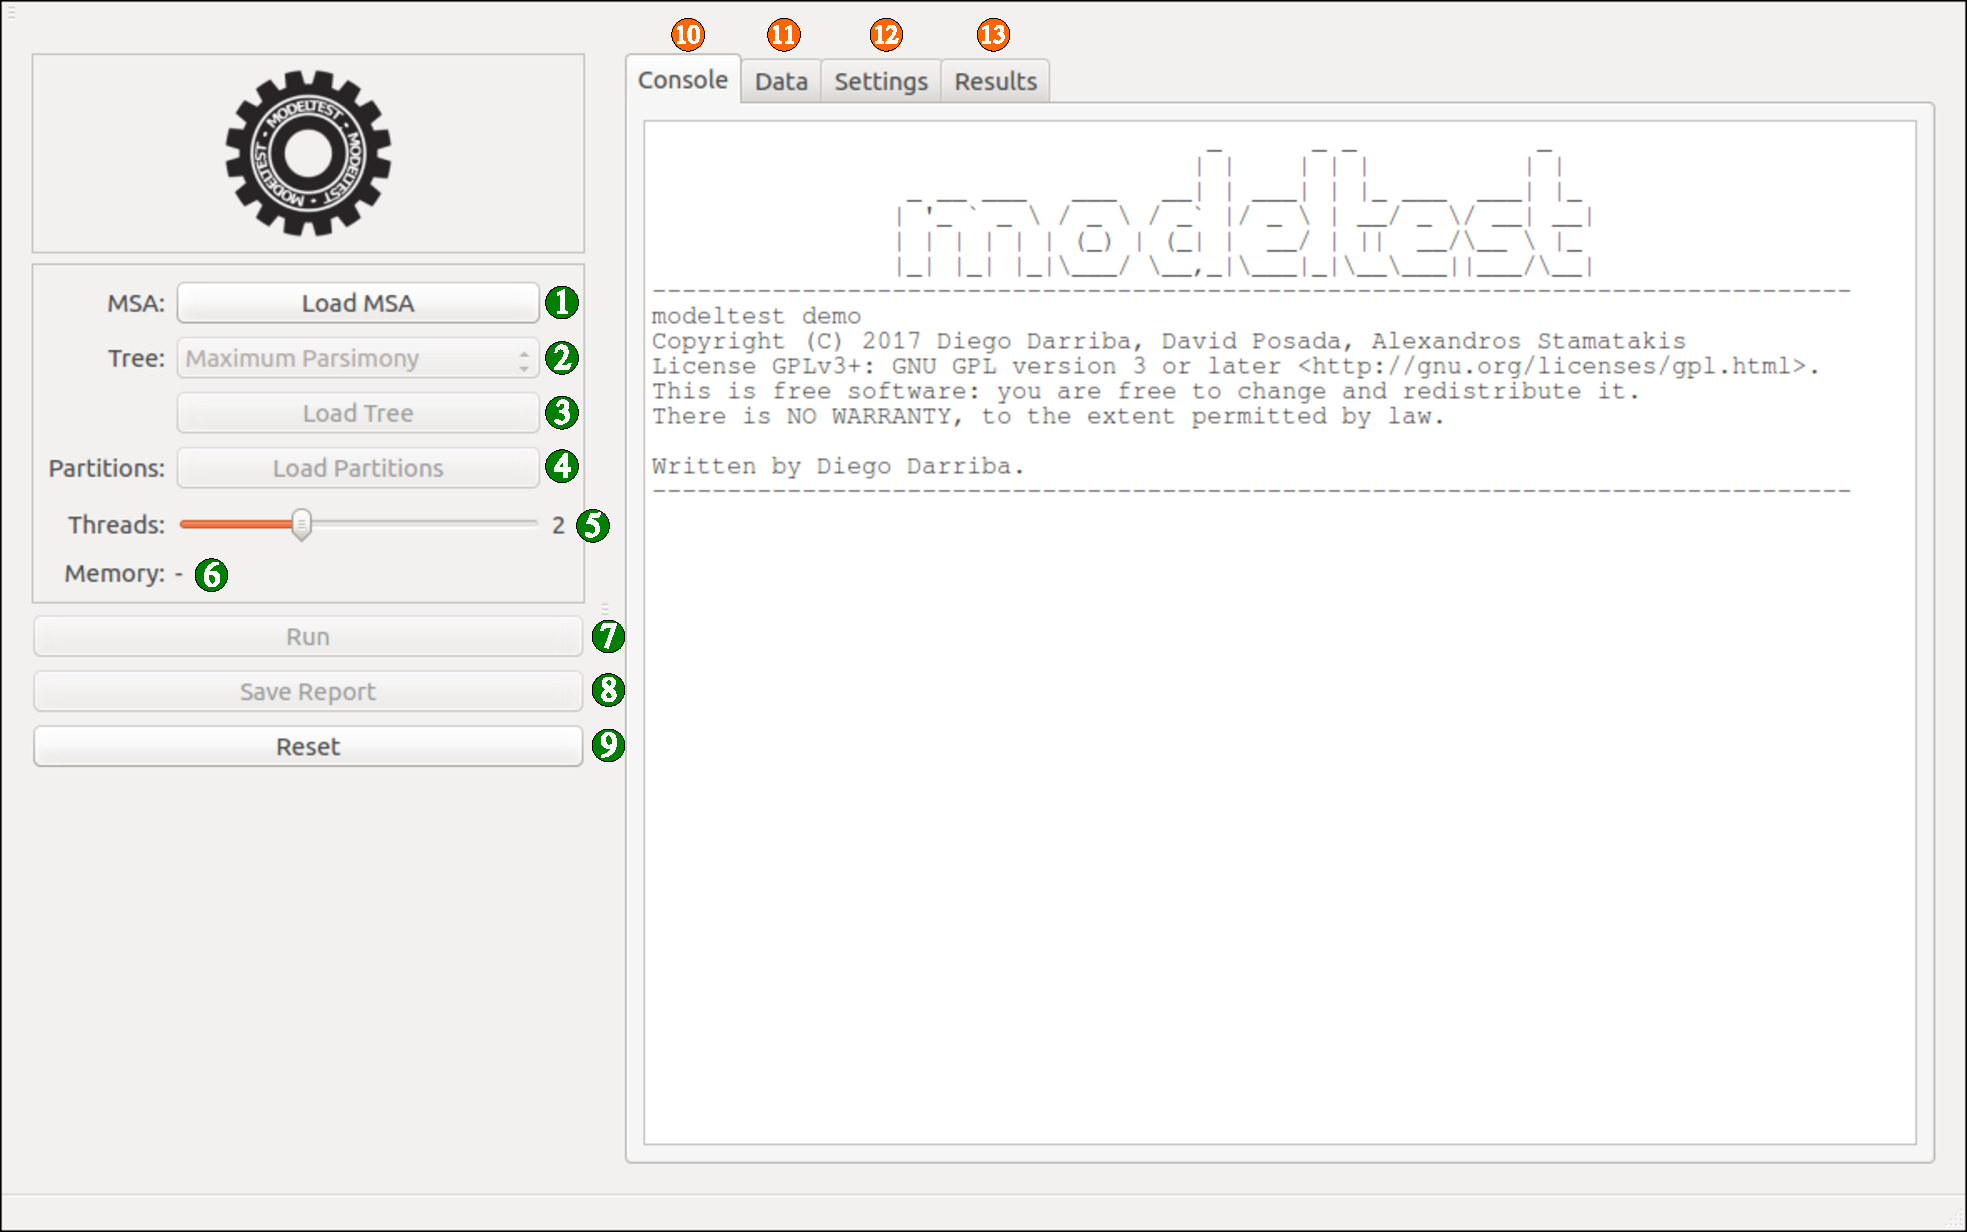
\includegraphics[width=.9\textwidth]{images/main-window}
\end{center}

\item Load an input alignment file using the {\bf File/Load Alignment} option.

\item Go to {\bf Analysis/Compute Likelihood Scores} and select the candidate models and the options for model optimization (optionally you can set a base topology from a file). Press Enter or the {\bf Compute Likelihoods} button.

\begin{center}
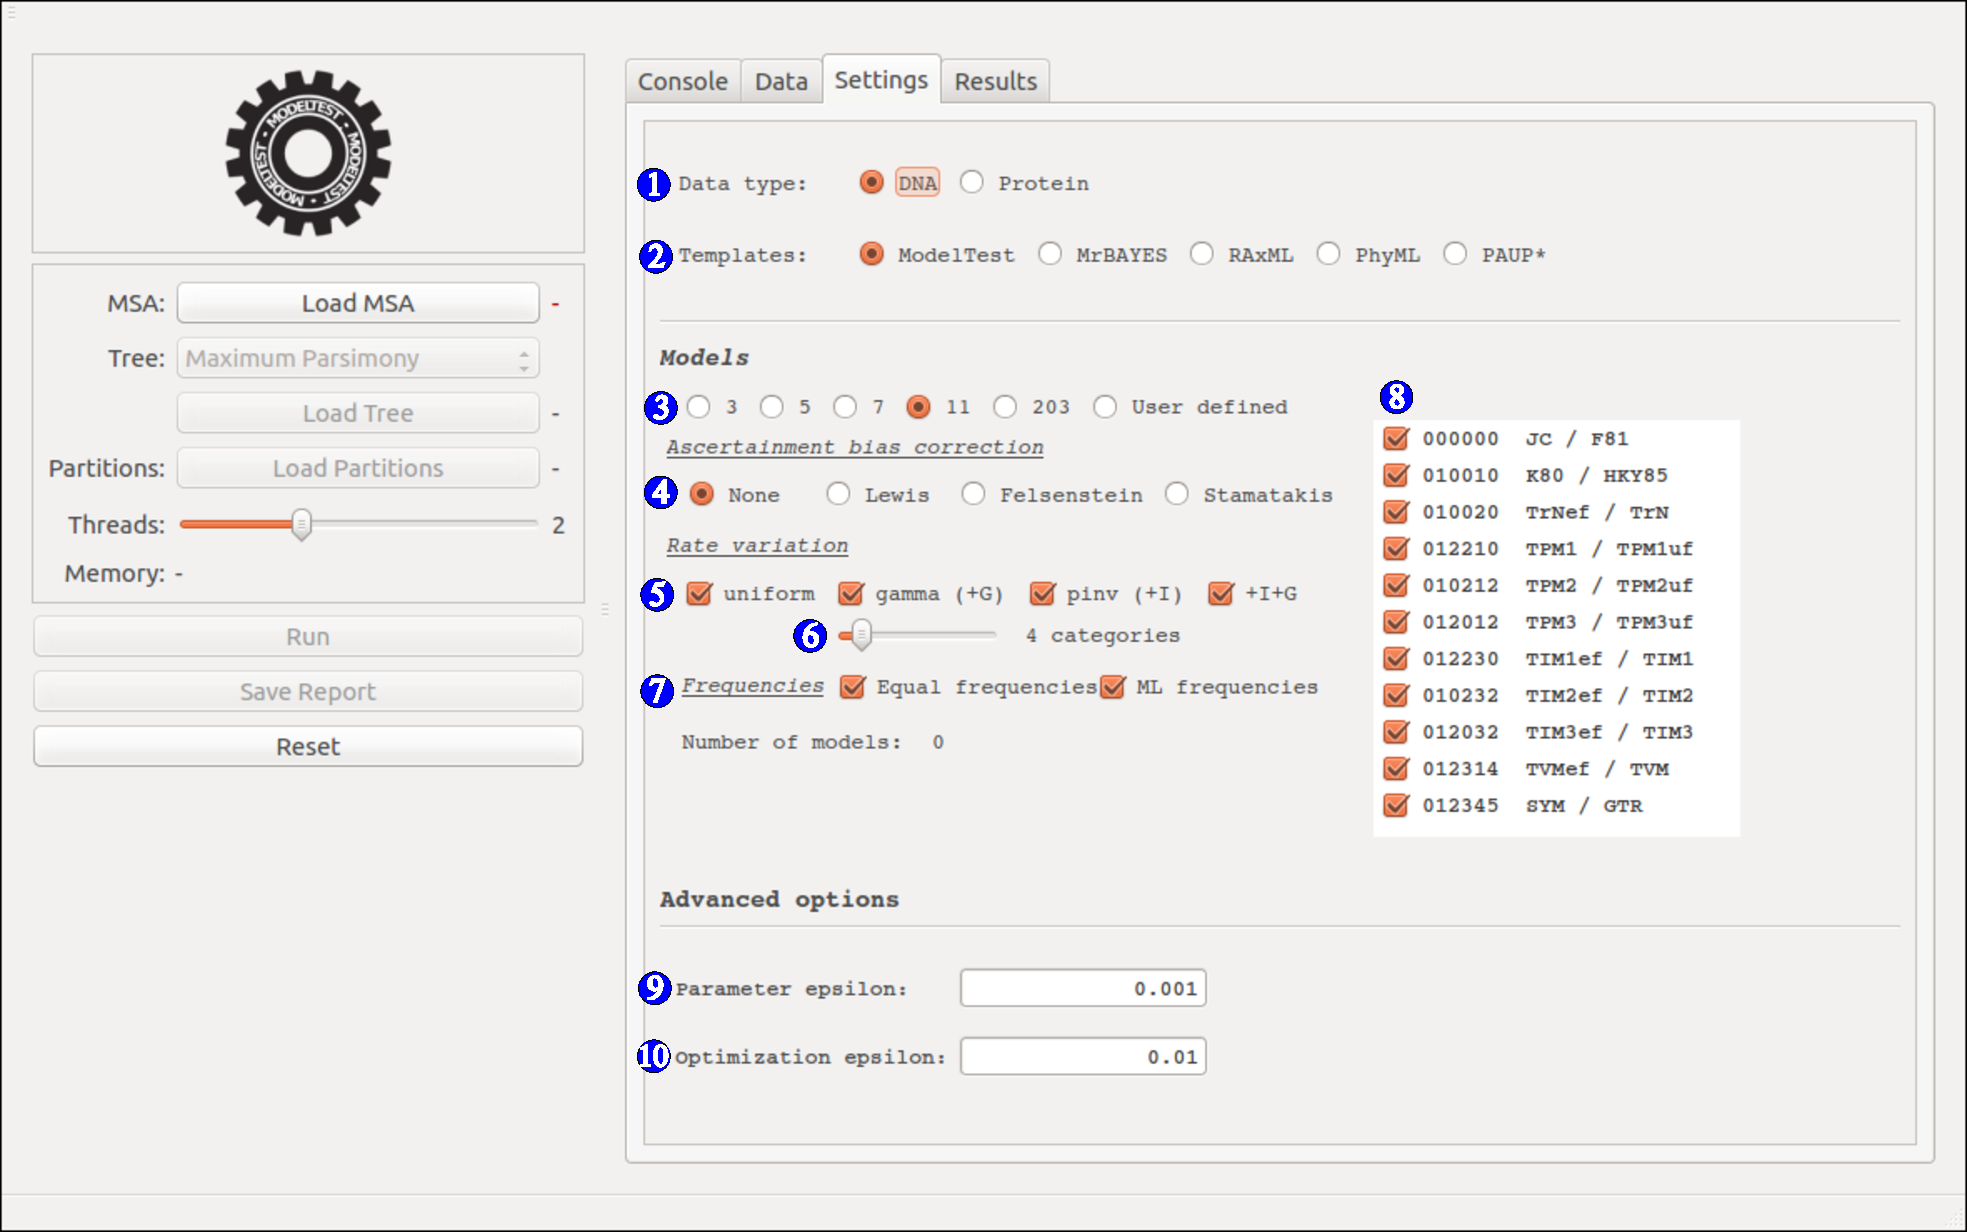
\includegraphics[width=.6\textwidth]{images/lkl-settings}
\end{center}

\item Perform statistical selection among the optimized models. For example, we can calculate the Bayesian Information Criterion using {\bf Analysis/Do BIC calculations...} option, or any other. You can find a Criteria comparison in terms of accuracy in the \href{http://www.nature.com/nmeth/journal/v9/n8/extref/nmeth.2109-S1.pdf}{supplementary material} of the \href{http://www.nature.com/nmeth/journal/v9/n8/full/nmeth.2109.html}{jModelTest publication}.

\begin{center}
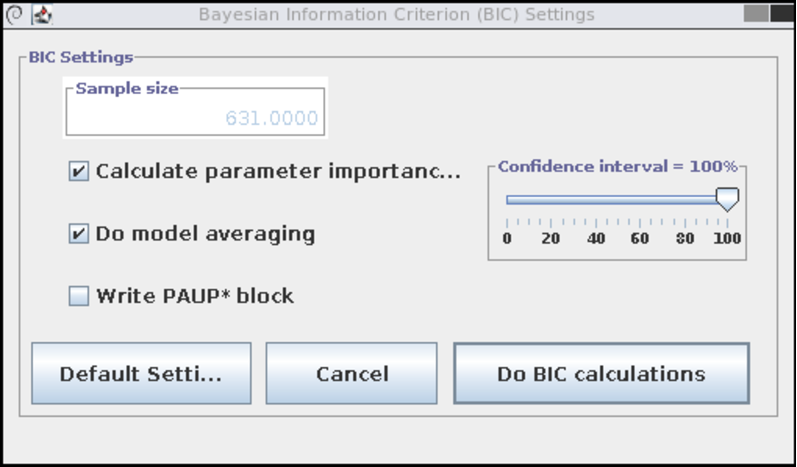
\includegraphics[width=.6\textwidth]{images/bic}
\end{center}

The results will be shown in the main console.

\item Take a look at the results table in {\bf Results/Show results table}. Best model is the one with the lowest criterion value (BIC column in the example) and therefore delta = 0.

\begin{center}
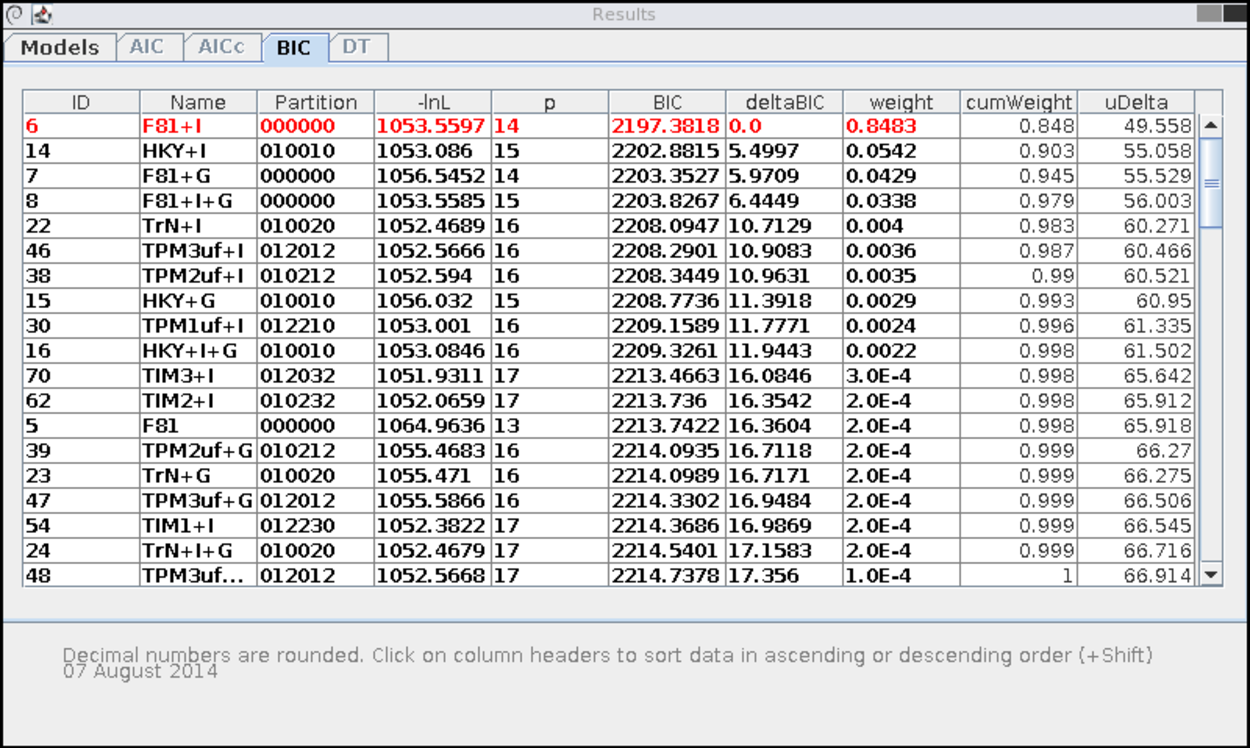
\includegraphics[width=.9\textwidth]{images/results}
\end{center}

\item Build a consensus tree from a given selection criteria using {\bf Analysis/Model-averaged phylogeny}:

\begin{center}
\includegraphics[width=.6\textwidth]{images/consensus}
\end{center}

\item Finally, you can save the results displayed in the main console using {\bf Edit/Save console}. Alternatively, you can get a formatted HTML document using {\bf Results/Build HTML log}:

\begin{center}
\includegraphics[width=.9\textwidth]{images/html-log}
\end{center}

Take a look at Section \ref{sec:gui} for further information.

\end{enumerate}

\subsubsection{Command Console Interface}

\begin{enumerate}
\item Execute the following command line:

\begin{lstlisting}
$ ./modeltest-cmd -i example-data/dna/aP6.fas -h uigf -f ef
\end{lstlisting}

This will test all 88 models (gamma models with 4 rate categories), and then perform the model selection using Akaike (AIC) and Bayesian (BIC) criteria.

See Section~\ref{sec:arguments} for information about supported arguments.

\item This will generate the following output:

\begin{enumerate}

\item Header:

\begin{lstlisting}
                                    _      _ _            _   
                                    | |    | | |          | |  
                 _ __ ___   ___   __| | ___| | |_ ___  ___| |_ 
                | '_ ` _ \ / _ \ / _` |/ _ \ | __/ _ \/ __| __|
                | | | | | | (_) | (_| |  __/ | ||  __/\__ \ |_ 
                |_| |_| |_|\___/ \__,_|\___|_|\__\___||___/\__|
--------------------------------------------------------------------------------
modeltest 0.1.0
Copyright (C) 2017 Diego Darriba, David Posada, Alexandros Stamatakis
License GPLv3+: GNU GPL version 3 or later <http://gnu.org/licenses/gpl.html>.
This is free software: you are free to change and redistribute it.
There is NO WARRANTY, to the extent permitted by law.

Written by Diego Darriba.
--------------------------------------------------------------------------------
\end{lstlisting}

\item Architecture options:

\begin{lstlisting}
Arch:           xxx
Physical cores: 2
Logical cores:  4
Memory:         3.57GB
Extensions:     AVX

\end{lstlisting}

\item Execution options:

\begin{lstlisting}
--------------------------------------------------------------------------------
Input data:
  MSA:        example-data/dna/aP6.fas
  Tree:       Maximum parsimony
    file:     -
  #taxa:      6
  #sites:     631
  #patterns:  28

Output:
  Log:           test.log
  Starting tree: test.tree
  Results:       test.out

Selection options:
  # dna schemes:      11
  # dna models:       88
  include model parameters:
    Uniform:         true
    p-inv (+I):      true
    gamma (+G):      true
    both (+I+G):     true
    fixed freqs:     true
    estimated freqs: true
    #categories:     4
  asc bias:           none
  epsilon (opt):      0.01
  epsilon (par):      0.01

Additional options:
  verbosity:        very low
  threads:          1/2
  RNG seed:         12345
  subtree repeats:  enabled
--------------------------------------------------------------------------------
modeltest was called as follows: 
>> src/modeltest-cmd -i example-data/dna/aP6.fas -h uifg -f fe -o test 
\end{lstlisting}

\item Real time optimization results (progress):

\begin{lstlisting}
Partition 1/1

 ----ID---  ----MODEL---- ---Time--- -Elapsed--- -------LnL------- -Alpha- -P-inv-
    1/88   JC             0h:00:00   0h:00:00           -1115.1193       -       -
    2/88   JC+I           0h:00:00   0h:00:00           -1103.3444       -  0.9082
    3/88   JC+G           0h:00:00   0h:00:00           -1106.6136  0.0200       -
    4/88   JC+I+G         0h:00:00   0h:00:00           -1103.6235  1.1674  0.8542
    5/88   F81            0h:00:00   0h:00:00           -1065.0339       -       -
    6/88   F81+I          0h:00:00   0h:00:00           -1053.6319       -  0.9032
    7/88   F81+G          0h:00:00   0h:00:00           -1056.6126  0.0200       -
    8/88   F81+I+G        0h:00:00   0h:00:00           -1053.8953  1.1494  0.8460

...

   85/88   GTR            0h:00:00   0h:00:01           -1063.2358       -       -
   86/88   GTR+I          0h:00:00   0h:00:01           -1051.9056       -  0.9001
   87/88   GTR+G          0h:00:00   0h:00:01           -1054.7872  0.0200       -
   88/88   GTR+I+G        0h:00:00   0h:00:01           -1052.1689  1.1396  0.8417
 ----ID---  ----MODEL---- ---Time--- -Elapsed--- -------LnL------- -Alpha- -P-inv-

Computation of likelihood scores completed. It took 0h:00:01
\end{lstlisting}

\item Selected Information Criteria (best model and all models sorted according to each criterion):

\begin{lstlisting}
BIC       model              K            lnL          score          delta    weight
--------------------------------------------------------------------------------
       1  F81+I              4     -1053.6319      2191.0788         0.0000    0.8565
       2  HKY+I              5     -1053.1557      2196.5737         5.4949    0.0549
       3  F81+G              4     -1056.6126      2197.0401         5.9613    0.0435
       4  F81+I+G            5     -1053.8953      2198.0529         6.9741    0.0262
       5  TrN+I              6     -1052.6019      2201.9134        10.8346    0.0038
       6  TPM2uf+I           6     -1052.6600      2202.0296        10.9507    0.0036
       7  HKY+G              5     -1056.0996      2202.4615        11.3827    0.0029
       8  TPM3uf+I           6     -1052.9534      2202.6164        11.5376    0.0027
       9  TPM1uf+I           6     -1053.0742      2202.8579        11.7791    0.0024
      10  HKY+I+G            6     -1053.4340      2203.5777        12.4988    0.0017
--------------------------------------------------------------------------------
Best model according to BIC
---------------------------
Model:              F81+I
lnL:                -1053.6319
Frequencies:        0.4253 0.1506 0.2010 0.2232 
Subst. Rates:       1.0000 1.0000 1.0000 1.0000 1.0000 1.0000 
Inv. sites prop:    0.9032
Gamma shape:        -
Score:              2191.0788
Weight:             0.8565
---------------------------
Parameter importances
---------------------------
P.Inv:              0.9244
Gamma:              0.0471
Gamma-Inv:          0.0282
Frequencies:        1.0000
---------------------------
Model averaged estimates
---------------------------
P.Inv:              0.9031
Alpha:              0.0200
Alpha-P.Inv:        1.1502
P.Inv-Alpha:        0.8459
Frequencies:        0.4253 0.1506 0.2010 0.2232 

Commands:
  > phyml  -i example-data/dna/aP6.fas -m 000000 -f m -v e -a 0 -c 1 -o tlr
  > raxmlHPC-SSE3 -s example-data/dna/aP6.fas -c 1 -m GTRCATIX --JC69 -n EXEC_NAME -p PARSIMONY_SEED
  > paup -s example-data/dna/aP6.fas
  > iqtree -s example-data/dna/aP6.fas -m F81+I
\end{lstlisting}

\item Consensus tree of the optimized phylogenies using the criterion weights:

\begin{lstlisting}
---------------------------------------------------------------
*                                                             *
*                    MODEL AVERAGED PHYLOGENY                 *
*                                                             *
---------------------------------------------------------------

Selection criterion: . . . . AIC
Confidence interval: . . . . 1.00
Consensus type:. . . . . . . 50% majority rule


Using 24 models in the 1.00 confidence interval = F81+I HKY+I F81+I+G HKY+I+G F81+G GTR+I HKY+G GTR+I+G GTR+G F81 HKY GTR JC+I K80+I JC+I+G K80+I+G JC+G K80+G SYM+I SYM+I+G SYM+G JC K80 SYM

Bipartitions included in the consensus tree

    123456
    ****** ( 1.0 )
    ****-- ( 1.0 )
    **---- ( 0.94244 )
    --**-- ( 1.0 )


                        +-----------6 P4
                      +-8
                      | +----------------5 P5
+---------------------9
|                     |  +-4 P1
|                     +--7
|                        +----------3 P6
|
+------2 P2
|
+---------------------------1 P3


(P3:0.016613,P2:0.004598,((P6:0.006790,P1:0.000000)1.00:0.002046,(P5:0.010191,P4:0.007198)0.94:0.001510)1.00:0.012665);

Note: this tree is unrooted. Branch lengths are the expected number of substitutions per site. Labels next to parentheses represent phylogenetic uncertainty due to model selection (see documentation)
\end{lstlisting}

\item Also a HTML log is automatically stored in the ``log'' directory.

\end{enumerate}
\end{enumerate}

\subsection{High Performance Environments}

\subsubsection{Shared memory architectures (multicore systems)}

Both the GUI and Console interfaces can be used for shared memory architectures. See Graphical User Interface or Command Console Interface. In some dedicated HPC environments you can only use the console interface, for example when using a bath-queuing system like Oracle Grid Engine. Additionally, in the console version you can specify the number of threads you want to use using the -tr'' option. By default, the total number of cores in the machine is used.

\subsubsection{Distributed memory architectures (HPC clusters)}

\begin{enumerate}
\item Besides the multithreading support, it is possible to run jModelTest in a cluster. This feature has been implemented using a Java message-passing (MPJ) library, MPJ Express (http://mpj-express.org/). To execute jModelTest in a cluster environment you have to:

\begin{lstlisting}
$ export $JMODELTEST_HOME=[path_to_jModelTest]
$ cd $JMODELTEST_HOME
$ tar zvxf mpj.tar.gz
$ export MPJ_HOME=$JMODELTEST_HOME/mpj
$ export PATH=$MPJ_HOME/bin:$PATH
$ cp $JMODELTEST_HOME/extra/machines $JMODELTEST_HOME
\end{lstlisting}

You can also add the last two lines to ~/.bashrc to automatically set these variables at console startup.

\item \$JMODELTEST\_HOME/machines file contains the set of computing nodes where the mpj processes will be executed. By default it points to the localhost machine, so you should change it if you want to run a parallel execution over a cluster machine, just writing on each line the particular computing nodes (e.g. see filecluster8.conf.template).

\item Start the MPJ Express daemons:

\begin{lstlisting}
$ mpjboot machines
\end{lstlisting}

The application ``mpjboot'' should be in the execution path (it is located at \$MPJ\_HOME/bin). A ssh service must be running in the machines listed in the machines file. Moreover, port 10000 should be free. For more details refer to the MPJ Express documentation.

\item Run jModelTest. For this, the jModelTest distribution provides a bash script: 'runjmodeltest-cluster.sh'

The basic syntax is:

./runjmodeltest-cluster.sh \$NUMBER\_OF\_PROCESSORS \$APPLICATION\_PARAMETERS

\begin{lstlisting}
$ ./runjmodeltest-cluster.sh 2 -d example-data/aP6.fas -s 11 -i -g 4 -f -AIC -a
\end{lstlisting}

\end{enumerate}
